\documentclass[12pt]{article}
	
\usepackage[margin=1in, left=0.6in, right=0.6in]{geometry}
\usepackage{fancyhdr}	% header
\usepackage{hyperref} % links


\usepackage{amsmath,amsthm,amssymb}	%math stuff
\usepackage{graphicx} \graphicspath{ {./images/} }
\usepackage{setspace} % increase line spacing
\usepackage{tabularx} % long tables
\usepackage{enumitem} % labelling itmes
\usepackage{color, soul}
\usepackage{lmodern} % bolding \texttt{}
\usepackage[T1]{fontenc} % for {} in \texttt{}
\usepackage{listings}
\usepackage[table]{xcolor}

\definecolor{dkgreen}{rgb}{0,0.6,0}
\definecolor{gray}{rgb}{0.5,0.5,0.5}
\definecolor{mauve}{rgb}{0.58,0,0.82}
\definecolor{backcolour}{rgb}{0.95,0.95,0.92}

\setlength{\parindent}{0pt}

\pagestyle{fancy}
\fancyhead[LO,L]{CSCB63 A3}
\fancyhead[CO,C]{Stephen Guo}
\fancyhead[RO,R]{1006313231}
\fancyfoot[LO,L]{}
\fancyfoot[CO,C]{\thepage}
\fancyfoot[RO,R]{}

\newcommand{\N}{\mathbb{N}}
\newcommand{\R}{\mathbb{R}}
\newcommand{\Rplus}{\mathbb{R}^{+}}
\newcommand{\bigbracket}[1]{\big(#1\big)}
\newcommand{\Bigbracket}[1]{\Big(#1\Big)}
\newcommand{\floorSurround}[1]{\left\lfloor#1\right\rfloor}
\newcommand{\ceilingSurround}[1]{\left\lceil#1\right\rceil}
\newcommand{\code}[1]{{\ttfamily \fontseries{b}\selectfont #1}}
\definecolor{codegray}{gray}{0.9}
\def \calO {\mathcal{O}}
\newcommand{\bigO}[1]{\ensuremath{\calO(#1)}}
\renewcommand{\qed}{\hfill$\blacksquare$}
\newenvironment{proofindent}{\vspace*{2mm}\hfill\begin{minipage}{\dimexpr\textwidth-10mm}}{\end{minipage}}

\everymath{\displaystyle}

\begin{document}
%----------------------------------------------------------------------------------
%                              Table of Contents
%----------------------------------------------------------------------------------
\begin{center}
	\hypertarget{toc}{\LARGE \noindent \underline{\textbf{Table of Contents}}}\\
\end{center}

\noindent \hyperlink{1}{\textbf{Question 1:}}
\vspace{1mm}
\hrule
\vspace{1mm} \leavevmode \\

\noindent {\textbf{Question 2:}}
\vspace{1mm}
\hrule
\vspace{1mm} \leavevmode \\
\noindent\hyperlink{2.1}{(a)}\\
\hyperlink         {2.2}{(b)}\\
\hyperlink         {2.3}{(c)}\\
\hyperlink         {2.4}{(d)}\\
\hyperlink         {2.5}{(e)}\\


\noindent {\textbf{Question 3:}}
\vspace{1mm}
\hrule
\vspace{1mm}
\noindent\hyperlink{3.1}{(a)}\\
\hyperlink         {3.2}{(b)}\\
\hyperlink         {3.3}{(c)}\\
\newpage

%{\setstretch{1.5}$\begin{array}{r@{}>{\displaystyle}l}  \end{array}$}
%----------------------------------------------------------------------------------
%                                   Questions
%----------------------------------------------------------------------------------
\setstretch{1.2}
%----------------------------------------------------------------------------------
% !                                    1
%----------------------------------------------------------------------------------
\noindent \hyperlink{toc}{\hypertarget{1}{\LARGE \underline{\textbf{Question 1.}}}}
\\\\
Let $n = $ num of elements in array,\\$m = $ size of array\\
Let $\phi(h) = 4n - 2m$\\
$\phi(h_0) = 4(0) - 2(0) = 0$ since we start off with no elements and an empty array\\
$\phi(h_i) \geq 0$\\
This is because the array is resized after there is more than $m$ elements. So after the resize, there will be $n+1$ elements, with the array of size $\ceilingSurround{1.5n}$. $\ceilingSurround{4(n+1)} \geq 2\ceilingSurround{1.5n}$. For any operation after that, the number of elements increases, but the size of array stays the same.
\\\\
Appending an element:\\
Case 1: $n < m$

\begin{proofindent}
	The actual cost is 1, since only one element is added to the array.\\
	{\setstretch{1.5}$\begin{array}{r@{}>{\displaystyle}l}  
		\Delta\phi(h) &{}= 4(n+1) - 2(m) - (4n - 2m)\\
		&{}=4 \\
	\end{array}$}\\
	Therefore amortized time $= 1+4 \in \calO(1)$
\end{proofindent}
\\\\\\
Case 2: $n = m$

\begin{proofindent}
	The actual cost is $n+1$, since the entire array is copied plus the new element.\\
	{\setstretch{1.5}$\begin{array}{r@{}>{\displaystyle}l}  
		\Delta\phi(h) &{}= 4(n+1)-2\ceilingSurround{1.5n} - (4n - 2n)\\
		&{}=4 - 2\ceilingSurround{1.5n} + 2n\\
		&{}=\left\{
		\begin{aligned}
			\ 4 - 3n + 2n & \hspace*{3mm}\text{ if } n \text{ is even} \\
			\ 4 - (3n+1) + 2n & \hspace*{3mm}\text{ if } n \text{ is odd} \\
		\end{aligned}
		\right. \\
		&{}=\left\{
		\begin{aligned}
			\ 4 - n & \hspace*{3mm}\text{ if } n \text{ is even} \\
			\ 3 - n & \hspace*{3mm}\text{ if } n \text{ is odd} \\
		\end{aligned}
		\right.
	\end{array}$}\ \\\\\\
	{\setstretch{1.5}$\begin{array}{r@{}>{\displaystyle}l}  
		\text{Amortized Time} &{}= \left\{
			\begin{aligned}
				\ n + 4 - n & \hspace*{3mm}\text{ if } n \text{ is even} \\
				\ n + 3 - n & \hspace*{3mm}\text{ if } n \text{ is odd} \\
			\end{aligned}
			\right. \\
		&{}= \left\{
			\begin{aligned}
				\  4  & \hspace*{3mm}\text{ if } n \text{ is even} \\
				\ 3 & \hspace*{3mm}\text{ if } n \text{ is odd} \\
			\end{aligned}
			\right.\\
		&{}\in  \calO(1) \\
	\end{array}$} 
\end{proofindent}

\newpage
%----------------------------------------------------------------------------------
% !                                    2
%----------------------------------------------------------------------------------
{{\LARGE \noindent \underline{\textbf{Question 2.}}}}
\\\\
\noindent \hyperlink{toc}{\hypertarget{2.1}{(a)}}\\
\begin{center}
	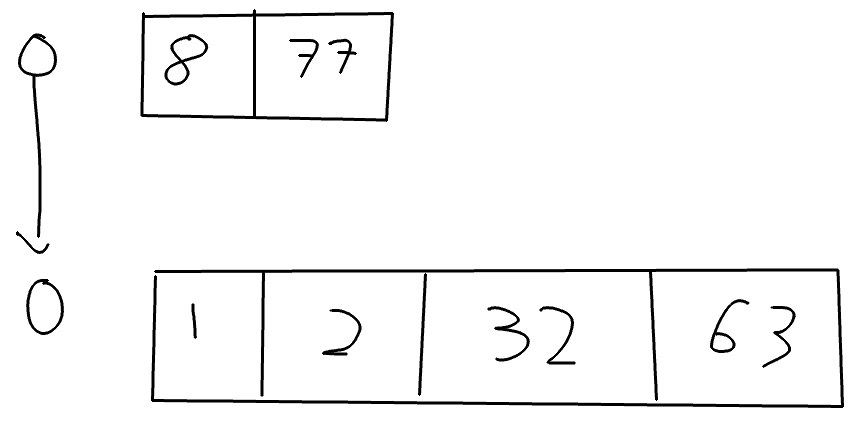
\includegraphics[width=7cm]{CSCB63_A3_2.png}
\end{center}
\noindent \hyperlink{toc}{\hypertarget{2.2}{(b)}}\\
% 
Let $I_n$ denote the set of bit positions in the binary representation of $n$ that contain the value of 1. Then in the data structure, those positions in $I_n$ will also be where the elements are in the data structure.\\
Let $I_n = \{j_1, j_2, \cdots, j_p\}$
\\\\
The worst case for \code{SEARCH(k)} is if \code{k} is not in the data structure. So the total time complexity is:
$$ \sum_{i=1}^{p} \bigbracket{\log_2(2^{j_i}) + 1} = \left(\sum_{i=1}^{p} {j_i}\right) + p$$

\noindent \hyperlink{toc}{\hypertarget{2.3}{(c)}}\\
The worst case for \code{INSERT(k)} is if all $j_i \in I_n$ needs to be merged. So the total time complexity is:
$$\sum_{i=1}^{p} 2^{j_i} = n$$
\newpage
\noindent \hyperlink{toc}{\hypertarget{2.4}{(d)}}\\
*Assuming creating an array of size 1, and inserting it to the beginning of the linked list costs 1. Merging 2 arrays costs the sum of the 2 array sizes.
\\\\
In the following table, we will have the insertion vs total costs.
\begin{center}
	\begin{tabular}{|c|c|c|c|}
		\hline \cellcolor{gray!25}Number of insertions & \cellcolor{gray!25}Cost of Current Operation & \cellcolor{gray!25}Total Cost & \cellcolor{gray!25}\texttt{floor(n * log(n) + 2*n)} \\
		\hline\hline
		\texttt{1}  & \texttt{2}  & \texttt{2}  & \hl{\texttt{2}}  \\\hline
		\texttt{2}  & \texttt{4}  & \texttt{6}  & \hl{\texttt{6}}  \\\hline
		\texttt{3}  & \texttt{2}  & \texttt{8}  & \texttt{10} \\\hline
		\texttt{4}  & \texttt{8}  & \texttt{16} & \hl{\texttt{16}} \\\hline
		\texttt{5}  & \texttt{2}  & \texttt{18} & \texttt{21} \\\hline
		\texttt{6}  & \texttt{4}  & \texttt{22} & \texttt{27} \\\hline
		\texttt{7}  & \texttt{2}  & \texttt{24} & \texttt{33} \\\hline
		\texttt{8}  & \texttt{16} & \texttt{40} & \hl{\texttt{40}} \\\hline
		\texttt{9}  & \texttt{2}  & \texttt{42} & \texttt{46} \\\hline
		\texttt{10} & \texttt{4}  & \texttt{46} & \texttt{53} \\\hline
		\texttt{11} & \texttt{2}  & \texttt{48} & \texttt{60} \\\hline
		\texttt{12} & \texttt{8}  & \texttt{56} & \texttt{67} \\\hline
		\texttt{13} & \texttt{2}  & \texttt{58} & \texttt{74} \\\hline
		\texttt{14} & \texttt{4}  & \texttt{62} & \texttt{81} \\\hline
		\texttt{15} & \texttt{2}  & \texttt{64} & \texttt{88} \\\hline
		\texttt{16} & \texttt{32} & \texttt{96} & \hl{\texttt{96}} \\\hline
		% &&\\\hline
	\end{tabular}
\end{center}
It is clear that the total cost is always $\leq n \log_2(n) + 2n$\\
% So we have Total Amortized Cost $ = \frac{n \log_2(n) + 2n}{n} = \log_2(n) + 2 \in \calO(\log_2 n)$ 
{$$\begin{array}{r@{}>{\displaystyle}l}
	\text{Total Amortized Cost} & {} = \frac{n \log_2(n) + 2n}{n} \\[0.5em]
	&{} = \log_2(n) + 2 \\[0.5em]
	&{} \in \calO(\log_2 n)\\
\end{array}$$}

\newpage
\noindent \hyperlink{toc}{\hypertarget{2.5}{(e)}}\\
Lets charge for each operation $\floorSurround{\log_2n} + 4$.
\\\\
Proving total credits $\geq 0$:\\
\begin{center}
	\begin{tabular}{|c|c|c|c|}
		\hline \cellcolor{gray!25}Insertions & \cellcolor{gray!25}Cost & \cellcolor{gray!25}Credits Charged & \cellcolor{gray!25}Credits Left \\
		\hline\hline
		\texttt{1}  & \texttt{2}  & \texttt{4} & \hl{\texttt{2}} \\\hline
		\texttt{2}  & \texttt{4}  & \texttt{5} & \hl{\texttt{3}} \\\hline
		\texttt{3}  & \texttt{2}  & \texttt{5} & \texttt{6}      \\\hline
		\texttt{4}  & \texttt{8}  & \texttt{6} & \hl{\texttt{4}} \\\hline
		\texttt{5}  & \texttt{2}  & \texttt{6} & \texttt{8}      \\\hline
		\texttt{6}  & \texttt{4}  & \texttt{6} & \texttt{10}     \\\hline
		\texttt{7}  & \texttt{2}  & \texttt{6} & \texttt{14}     \\\hline
		\texttt{8}  & \texttt{16} & \texttt{7} & \hl{\texttt{5}} \\\hline
		\texttt{9}  & \texttt{2}  & \texttt{7} & \texttt{10}     \\\hline
		\texttt{10} & \texttt{4}  & \texttt{7} & \texttt{13}     \\\hline
		\texttt{11} & \texttt{2}  & \texttt{7} & \texttt{18}     \\\hline
		\texttt{12} & \texttt{8}  & \texttt{7} & \texttt{17}     \\\hline
		\texttt{13} & \texttt{2}  & \texttt{7} & \texttt{22}     \\\hline
		\texttt{14} & \texttt{4}  & \texttt{7} & \texttt{25}     \\\hline
		\texttt{15} & \texttt{2}  & \texttt{7} & \texttt{30}     \\\hline
		\texttt{16} & \texttt{32} & \texttt{8} & \hl{\texttt{6}} \\\hline
		% &&\\\hline
	\end{tabular}
\end{center}
For all credits left, it is always $\geq \log_2(n) + 2$\\
Which is always $\geq 0$ for all $n \in \N^+$
\\\\
Since we charge $\floorSurround{\log_2n} + 4$ for each operation, therefore the Total Amortized Cost $\in \calO(\log_2 n)$
\\\\

\newpage
%----------------------------------------------------------------------------------
% !                                    3
%----------------------------------------------------------------------------------
{{\LARGE \noindent \underline{\textbf{Question 3.}}}}
\\\\
\noindent \hyperlink{toc}{\hypertarget{3.1}{(a)}}
\begin{center}
	The forest
after performing operations:
$\textsc{Union}(5,2)$,
$\textsc{MakeSet}(3)$,
$\textsc{MakeSet}(4)$,
$\textsc{Union}(3,4)$,
$\textsc{Union}(5,3)$,
$\textsc{MakeSet}(1)$,
$\textsc{MakeSet}(8)$,
$\textsc{Union}(1,8)$,
$\textsc{FindSet}(8)$,\\\ \\
	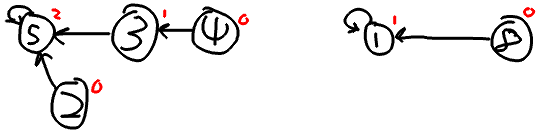
\includegraphics[width=10cm]{CSCB63_A3_3-1.png}
	\ \\\ \\\ \\
	The forest after performing operation: $\textsc{Union}(4,1)$.\\\ \\
	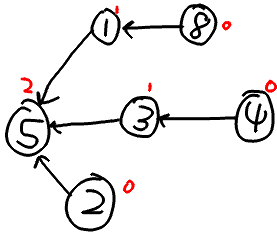
\includegraphics[width=5cm]{CSCB63_A3_3-2.png}
\end{center}
\noindent \hyperlink{toc}{\hypertarget{3.2}{(b)}}\\
Yes.\\
Let $P = \textsc{MakeSet(1), MakeSet(2), Union(1,2), MakeSet(3), Union(1,3)}$\\\\
Up until $\textsc{MakeSet(3)}$, The same number of nodes are accessed. \\
For $\textsc{Union(1,3)}$, the linked list must traverse through the node (1) and (2) to insert the node (3). For the tree, node (3) is directly pointed to node (1). This makes it so that the linked list accesses 1 extra time, which is node (2). 
\begin{center}
	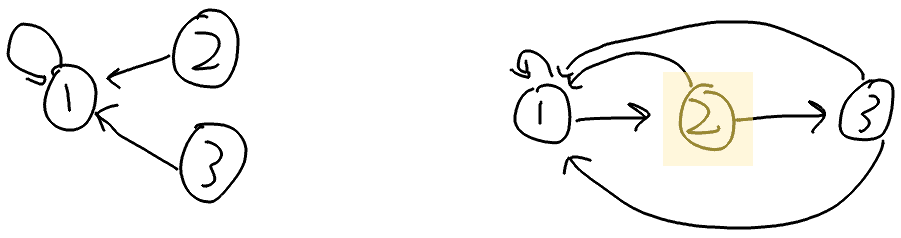
\includegraphics[width=12cm]{CSCB63_A3_3-3.png}
\end{center}
\newpage
\noindent \hyperlink{toc}{\hypertarget{3.3}{(c)}}\\
Yes.\\
Let $P = \textsc{MakeSet}(5), \textsc{MakeSet}(2), \textsc{Union}(5,2), \textsc{MakeSet}(3), \textsc{MakeSet}(4), \textsc{Union}(3,4), $\\ \textsc{Union}(2,3), \textsc{Find(4)}.
\begin{center}
	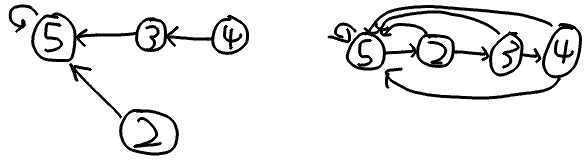
\includegraphics[width=12cm]{CSCB63_A3_3-4.png}
\end{center}
Up until \textsc{Union}(2,3), The tree has 1 less access than the linked list. This is because the linked list needs to update nodes (2), (3), and (4). For the tree, it just needs to access node (5) and (3).
\\\\
After \textsc{Find(4)}, the Tree needs to perform path compression, which requires access to nodes (4), (3), and (5). However for the linked list, It only needs to access node (4). Thus, the tree will have accessed 1 more node than the linked list.

\end{document}